% Part: sets-functions-relations
% Chapter: infinite
% Section: hilberts-hotel
%
\documentclass[../../../include/open-logic-section]{subfiles}

\begin{document}

\olfileid[ar]{sfr}{infinite}{hilbert}
\olsection{فندق هيلبرت}

لا ريب في أن مجموعة الأعداد الطبيعية لا نهائية. فإذا لم نرد أن \emph{نأخذ} الطبيعية معطاة لنا، وجب أولًا وصف المجموعة اللانهائية بعبارة لا تتوقف على ذكر الأعداد الطبيعية نفسها. ولهذا عرض هيلبرت في محاضرة سنة \OLClassicalDigits{1924} تصويرًا حسنًا، فدعانا إلى تخيل
\begin{quote}
[\ldots] فندق غرفه متناهية العدد، في كل غرفة منها نزيل واحد بعينه. فإذا تبادل النزلاء غرفهم على أي وجه، [على شرط] ألا يجتمع في غرفة أكثر من واحد، لم تخل غرفة؛ فلا يستطيع صاحب الفندق بهذه الوسيلة أن يفسح مكانًا لنزيل وافد [\ldots \textparagraph \ldots]

ولنفرض الآن غرف الفندق لا نهائية، مرقمة $\OLMathNumeral{1}$، و$\OLMathNumeral{2}$، و$\OLMathNumeral{3}$، و$\OLMathNumeral{4}$، و$\OLMathNumeral{5}$، \dots، وفي كل منها نزيل واحد. فإذا وفد نزيل جديد، كفى صاحب الفندق أن ينقل كل نزيل قديم إلى الغرفة التي يزيد رقمها واحدًا على رقم غرفته؛ فتخلو الغرفة~$\OLMathNumeral{1}$ للوافد.
\begin{center}
		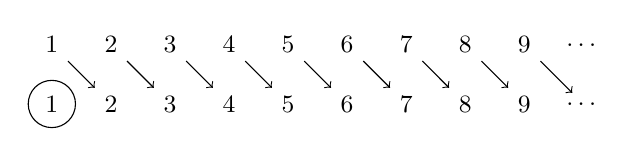
\begin{tikzpicture}[scale = .75]
		\foreach \x in {1, 2, 3, 4, 5, 6, 7, 8, 9}
		{
			\node (\x a) at (\x, 1) {\small{\x}};
			\node (\x b) at (\x, 2) {\small{\x}};
		}
		\node (dotsa) at (10, 1) {\small{\ldots}};
		\node (dotsb) at (10, 2) {\small{\ldots}};
		\draw[->] (1b)--(2a);
		\draw[->] (2b)--(3a);
		\draw[->] (3b)--(4a);
		\draw[->] (4b)--(5a);
		\draw[->] (5b)--(6a);
		\draw[->] (6b)--(7a);
		\draw[->] (7b)--(8a);
		\draw[->] (8b)--(9a);
		\draw[->] (9b)--(dotsa);
		\draw (1,1) circle (.4);
		\end{tikzpicture}
	\end{center}
 	(نشر في \citealt[ص~730]{EwaldSieg2013}؛ والمراد بقول الأصل «ترجمتنا» ترجمة محرري النص الإنجليزي)
\end{quote}
ومدار الأمر أن غرف فندق هيلبرت لا نهائية؛ بل نستطيع اتخاذ هذا التصوير حدًّا لمعنى اللانهاية. وهذا في الحقيقة نهج ديديكند؛ وإن قدمناه هنا على غير ترتيب التاريخ تقديمًا بيّنًا، لأن تعريف ديديكند يرجع إلى \citeyear{Dedekind1888}:

\begin{defn}\ollabel{defn:DedekindInfinite}
المجموعة $\OLId{latin-looped}{A}$ \emph{لانهائية بحسب ديديكند} إذا وفقط إذا وجدت !!a{injection} من~$\OLId{latin-looped}{A}$ إلى جزء حقيقي من~$\OLId{latin-looped}{A}$. أي يوجد $\OLId{latin-ordinary}{o} \in \OLId{latin-looped}{A}$ وتوجد !!a{injection} $\OLId{latin-ordinary}{f} \colon \OLId{latin-looped}{A} \to \OLId{latin-looped}{A}$ تحقق $\OLId{latin-ordinary}{o} \notin \ran{\OLId{latin-ordinary}{f}}$.
\end{defn}

\end{document}
